\documentclass{article}

\usepackage[utf8]{inputenc}

% Packages
\usepackage{amsmath,amssymb}
\usepackage{bm}% boldmath
\usepackage{listings} % Code block (source code) \begin{lstlisting} 
\usepackage{natbib}
\usepackage{graphicx}
\usepackage{lmodern}
\usepackage[usenames,dvipsnames,svgnames,table]{xcolor}
\usepackage[textwidth=16cm,textheight=23cm]{geometry}

%\usepackage{inconsolata} % New monospace font

% URL
\usepackage{url}
\usepackage[colorlinks=true, a4paper=true, pdfstartview=FitV, linkcolor=blue, citecolor=blue, urlcolor=blue]{hyperref}

% Figures
\usepackage[font=small, labelfont=bf]{caption}
\usepackage{subfig} % Subfigures. Uses \subfloat[captions text]{figure}

% Tables
\usepackage{booktabs}   % Allows the use of \toprule, \midrule and \bottomrule in tables for horizontal lines
\newcommand{\ra}[1]{\renewcommand{\arraystretch}{#1}} % spaces in tables

% Itemize
\usepackage{enumitem}

% Commands
%\newcommand{\code}[1]{\texttt{#1}} % \code{inline code}
\newcommand{\code}[1]{{\small\ttfamily #1}} % \code{inline code}
\newcommand{\expval}[1]{\langle #1 \rangle} %
\renewcommand{\theequation}{\arabic{section}.\arabic{equation}} % Book format equation
\renewcommand{\thefigure}{\arabic{section}.\arabic{figure}} % Book format figure
\renewcommand{\vec}[1]{{\bf #1}} % Lars likes this better than arrow

% Set page attribution
\setlength{\parindent}{0pt}


% PSTRICKS
\usepackage{pstricks,pst-node,pst-tree} % includes graph additions
\usepackage{pst-pdf} % Compiles the pictures
\usepackage{pst-node}
\usepackage{pst-plot}
\usepackage{pst-3dplot}
%\usepackage{pstricks-add,babel}




\lstset{
language=Python,                        % Code langugage
commentstyle=\color{gray},              % Comments font
basicstyle=\small\ttfamily,             % Code font, Examples: \footnotesize, \ttfamily
keywordstyle=\bfseries\color{blue},
stringstyle=\color{orange},
numbers=left,                           % Line nums position
numberstyle=\tiny,                      % Line-numbers fonts
stepnumber=1,                           % Step between two line-numbers
numbersep=5pt,                          % How far are line-numbers from code
frame=none,                             % A frame around the code
tabsize=4,                              % Default tab size
captionpos=b,                           % Caption-position = bottom
breaklines=true,                        % Automatic line breaking?
breakatwhitespace=false,                % Automatic breaks only at whitespace?
showspaces=false,                       % Dont make spaces visible
showstringspaces=false,                 % Dont make spaces visible in strings
showtabs=false,                         % Dont make tabls visible
belowskip=8pt,
morekeywords={range, xrange},
% backgroundcolor=\color{yellow}
% emph={[2]root,base}
% morekeywords={one,two,three,four,five,six,seven,eight,
}


%commentstyle=\color{gray},              % Comments font
%basicstyle=\small,                      % Code font, Examples: \footnotesize, \ttfamily



%basicstyle=\footnotesize\ttfamily,
%keywordstyle=\bfseries\color{green!40!black},
%commentstyle=\itshape\color{purple!40!black},
%identifierstyle=\color{blue},
%stringstyle=\color{orange},







% ***************************************************
% HEADER INFORMATION

\title{Ising Spin-Lattice Model}
\author{Molecular Statistics}
\date{2014}

% ***************************************************

\begin{document}


% ***************************************************
% BEGIN DOCUMENT
% ***************************************************


\maketitle

\section{Introduction}

\subsection{The Ising Model}

The Ising model is a mathematical representation of a magnetic solid.
The Ising model decribes the interaction of atomic magnetic dipoles (or spins) with its neighbors.
In this project, you will implement and simulate a 2D square-lattice Ising model.
In the 2D Ising model, magnetic spins are arranged on a 2D lattice (see Fig. \ref{fig:grid}).
Magnetic spin can be up or down (represented as 1 or -1). 

\begin{figure}[h!]
  \centering
  \subfloat[]{
    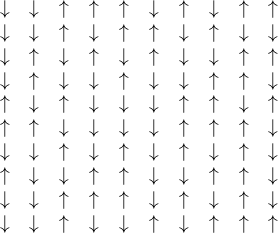
\includegraphics[width=0.3\textwidth]{lattice.png}
    \label{fig:grid}
  }
  \qquad % Spacing
  \qquad % Spacing
  \qquad % Spacing
  \subfloat[]{
    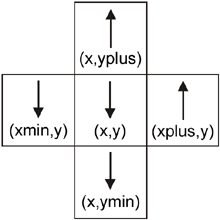
\includegraphics[width=0.2\textwidth]{neighbors.png}
    \label{fig:neighbors}
  }
  \caption{
    (a) An example of illustrating a 10x10 Ising spin lattice.
    (b) Illustrating the spin system $(x,y)$ and its neighbours used to calculate
    the interaction energy.
  }
\end{figure}

A Pythonic representation of a 5x5 spin-system could for instance be a 2D list or a 2D numpy-array with the following contents:

\begin{lstlisting}
lattice = [[ 1. -1.  1. -1.  1.],
           [-1.  1. -1.  1. -1.],
           [ 1. -1. -1.  1.  1.],
           [-1. -1.  1.  1. -1.],
           [ 1.  1. -1. -1.  1.]]
\end{lstlisting}

An easier way is to use the \code{np.random.randint()} function to generate a grid.

\subsection{Energy of the 2D Ising lattice} \label{section:energy}

Spins interact only with the four neighboring spins. The interaction energy between two neighbors is given by:
\begin{equation}
\epsilon_{ij} = -J \ S_i \ S_j
\end{equation} 

The value of S is either $1$ or $-1$, corresponding to a spin-up or spin-down state. $J$ is the interaction-constant.
The total energy of a spin lattice is thus:
\begin{equation}
E_{\mathrm{total}}=\sum^{\mathrm{neighbours}}_{ij} \epsilon_{ij} = -J \sum^{\mathrm{neighbours}}_{ij} \ S_i \ S_j
\end{equation}

where the sum runs over all unique neighboring pairs of magnetic dipoles.\\

The spin or the element in position $i$ will interact with four other elements.
The spin immediately above, below, to the right and to the left of that position as shown in figure \ref{fig:neighbors}.
The interaction energy \code{e} between these spins can be calculated in Python as:

\begin{lstlisting}[language=python]
e  = -J * lattice[x][y] * lattice[x][yplus]
e += -J * lattice[x][y] * lattice[x][ymin]
e += -J * lattice[x][y] * lattice[xplus][y]
e += -J * lattice[x][y] * lattice[xmin][y]
\end{lstlisting}

To simulate a real lattice, and not just a $N$x$N$ system, we will be using
periodic boundary conditions.
If an element is located on an edge we will make the element interact with the first element on the other side.
In the example above, the element with indexes (3, 0) will interact with (3, 4), (3, 1), (2, 0) and (4, 0).\footnote{Remember that Python indexing start at 0.}\\

If $J > 0$ the lowest energy configuration of the system is when all spins are aligned and have the same value.
This is called \textit{ferro-magnetism}.
We set $J = 1$ in the following, so all energies reported are in units of $J$.

\subsection{The Metropolis-Hastings algorithm}

The Metropolis-Hastings (MH) algorithm is a Monte Carlo algorithm that can be used to describe a probability distribution of the possible states of a system.
In this project, you will use the MH algorithm to determine the Boltzmann distribution of the 2D Ising model.\\

A system is in a state $K_n$.
A random Monte Carlo step then perturbs the system into a new proposed state, $K_{n+1}$.
The energy difference between the two states is $\Delta E = E_{n+1} - E_n$.
The probability of accepting the new state is then defined according to the Boltzmann distribution as:
\begin{equation}
P = \min \left[1, \exp \left(-\frac{\Delta E}{k_{\mathrm{B}}T}\right) \right]
\end{equation} 

If $\Delta E < 0$, the acceptance probability is $P = 1$, which means that new states with a lower energy are \textit{always} accepted.
Conversely, states with $\Delta E > 0 $ are only accepted with the probability described above.
Whether or not a move is accepted is evaluated using random numbers.
Python code for evaluating this could be:
\begin{lstlisting}
for n in range(n_steps):
    # Flip a spin
    dE = ...
    if dE < 0:
        # Accept change
    elif np.exp(-dE / (kB * T)) >= np.random.random():
        # Accept change
    else:
        # Reject change
        # Revert system back to old state
\end{lstlisting}

If the current energy is saved after each iteration in the loop, the distribution of the recorded energies corresponds to the Boltzmann Distribution (if the simulation is long enough).\\

It is common to set $k_{\mathrm{B}} = 1$ so that all temperatures reported are in units of $k_{\mathrm{B}}$.

\newpage
\subsection{Physical properties}

If you run a simulation as described in the previous chapter, you will obtain a probability distribution of the energy corresponding to the Boltzmann distribution.
The analytical expression for the Boltzmann distribution is:
\begin{equation}
\frac{N_i}{N} = \frac{1}{Z} g_i \exp \left[ \frac{-E_i}{k_{\mathrm{B}}T} \right]
\end{equation}

Where $\frac{N_i}{N}$ is the probability to observe the energy state $E_i$ which is $g_i$ degenerate.
$Z$ is the partition function.
Evaluation of the analytical expression is usually infeasible for large systems.
In these cases, Monte Carlo is a powerful tool to describe the Boltzmann distribution.

\subsubsection{Heat capacity}

The heat capacity describes how much the energy of the system changes with respect to a change in temperature.
For our system it can be defined as:
\begin{equation}
C_v = \left( \frac{J}{k_{\mathrm{B}}T} \right)^2 \left( \langle E^2 \rangle - \langle E \rangle^2 \right)
\end{equation}

%Here $N$ is width of the lattice (i.e. $N^2$ is the total number of spins).
$\langle E \rangle$ and $\langle E^2 \rangle$ are Boltzmann averages of the energy and \textit{squared} energy.
If you save the energy (and squared energy) after each iteration step throughout the simulation and take the average, you will obtain the correct values.
The energy $E$ is \textbf{not} the total energy, but the energy \textit{per} spin, i.e. $E = \frac{E_\mathrm{total}}{L^2}$,
where $L$ is the width of the lattice.

\subsubsection{Overall magnetization}

The magnetization is the average spin of the system, and is defined as;
\begin{equation}
M =\frac{1}{L^2} \sum_i S_i
\end{equation}

where $L$ is the width of the lattice.
At a low temperature $M$ will be close to either 1 or -1, depending on how the spins align.
Conversely, all spins are random in the high temperature limit, and the overall magnetization will be close to 0.

\subsubsection{Magnetic susceptibility}

The magnetic susceptibility describes how the magnetization changes with respect to a change in temperature.
This can be calculated as
\begin{equation}
\chi = \frac{J}{k_{\mathrm{B}}T} \left( \langle M^2 \rangle - \langle M \rangle^2 \right)
\end{equation}

where $\langle M \rangle$ and $\langle M^2 \rangle$ are calculated as averages over a simulation.

\subsubsection{Critical temperature}

The temperature $T_c = 2.269$ (the \textit{critical temperature}) is the highest temperature at which there can be a non-zero magnetization.
The system undergoes a phase transition if the temperature is changed across $T_c$, from being an ordered state to a disordered state.

\newpage
\subsection{PyPy}
PyPy is an alternative implementation of Python that functions similarly to Numba, which you have previously used via Anaconda.
Using PyPy instead of regular Python gives you around a factor of 6 increase in speed,
but it doesn't fully support NumPy or Matplotlib.
You can get around this by using \code{lists} instead of \code{ndarrays}, the \code{random} module instead of \code{numpy.random} and saving the simulation observables to a file and plotting it later.
Using PyPy isn't strictly necessary, but can help reduce your simulation time.
You can install it by executing the following in the terminal:

\begin{lstlisting}
sudo apt-get install pypy
\end{lstlisting}


Then execute your python code with \code{pypy <program.py>} instead of with Python.

\newpage
\section{Assignment}
\subsection{The 2D grid}

The central mathematical entity in your program is the 2D lattice.
Come up with a way to define a square 2D list (or Numpy array) containing randomly distributed values of -1 or 1.

\subsection{Calculating total energy}

In order to calculate the total energy of a system you have to sum up all unique pairs of interactions. Make a function called \code{calc\_energy()} that takes the lattice as argument:

\begin{lstlisting}
def calc_energy(lattice):
    energy = 0.0
    for x in range(len(lattice)):
        for y in range(len(lattice)):
            # Calculate xplus, xmin, yplus and ymin here
            # See fig. 2
            energy = energy + lattice[x][y] * ...
    return energy
\end{lstlisting}

See section \ref{section:energy} for hints on calculating the energy.
Test your code.
An $L$x$L$ lattice with all spins aligned should have the energy $-2L^2$.
Make sure you do not count the same interaction twice.\\

\subsection{Random Monte Carlo move (spin flip)}

Monte Carlo (MC) works by randomly perturbing a system (via a \textit{Monte Carlo move}).
The simplest MC move in the 2D Ising model is a spin flip of a randomly chosen dipole in the lattice.
A random move could for instance be carried out like this:

\begin{lstlisting}
x = np.random.randint(lattice_size)
y = np.random.randint(lattice_size)

grid[x][y] *= -1.0
\end{lstlisting}

This, of course, has to be carried out once every iteration.

\subsection{Implementing the Metropolis-Hastings algorithm}

An example of how to implement the MH algorithm is: 

\begin{lstlisting}
lattice = ...
for n in range(n_steps):
    e_old = calc_energy(lattice):
    # Flip a spin
    e_new = calc_energy(lattice):
    dE = e_new - e_old
    if dE <= 0:
        # Accept the change
    elif np.exp(-dE / T) >= np.random.random():
        # Accept the change
    else:
        # Reject the change
        # Revert system back to old state
        #   i.e. flip the same spin back.
\end{lstlisting}

\subsection{Incremental energy calculation}

If you followed the example in the last section, you calculated the energy by summing up all contributions twice in order to calculate the energy difference, $\Delta E$.
It is, however, only necessary to calculate the energy of the parts of the system that change (you only change the energy interaction between four spins).
This will make your program run orders of magnitudes faster.\\

Change your code so you only calculate the total energy once, right after you initialize the grid.
During the simulation you can then add $\Delta E$ to the energy every time a new state is accepted.
Test your implementation by printing and comparing the energy calculated throughout the simulation with the energy you get if you use you \code{calc\_energy(lattice)} function.\\

This step is required for a program that is fast enough to run simulations of adequate lengths.

\subsection{Calculating the heat capacity}

After every iteration step save the current energy and the square of the current energy.
When a simulation at a given temperature is over, calculate the mean energy and mean squared energy.
Use these to calculate the heat capacity.\\

Test your code by running a simulation with a 20x20 matrix, 100,000 steps and $T = 1.5$.
You should get a $C_v$ around 
0.0004 to 0.0005.
The $\langle E \rangle$ should be around -1.95 and $\langle E^2 \rangle$ around 3.8.\\

Remember to run a burn-in period of at least 100,000 steps before you start to record the average energy and squared energy.
Run your simulation a couple of times to account for statistical variation in the result.\\

Note that the heat capacity has a divergence around $T = 2.269$. See Fig. \ref{fig:heat}.
If you run a simulation around this temperature your results will vary quite a bit.

\subsection{Calculate overall magnetization}

The magnetization is the mean spin of the system.
After each iteration in your Monte Carlo simulation calculate the magnetization and save it.
If you have stored your lattice in a 2D numpy-array or a 2D list, you can use the following numpy function to calculate the magnetization:

\begin{lstlisting}[language=python]
M = np.mean(lattice)
\end{lstlisting}

This is, however, not the fastest way of calculating the magnetization.
Just as you did with the energy difference, you can calculate the change in magnetization each iteration and
add this to the magnetization. This will be much faster.
Test your code by running a simulation at a low temperature ($T < 1$) and a high temperature ($T > 3.0$).
In the low temperature limit you should get $\langle M \rangle = \pm 1$ and zero in the high temperature limit - see Fig. \ref{fig:magnetization}.

\begin{figure}[p]
  \centering
  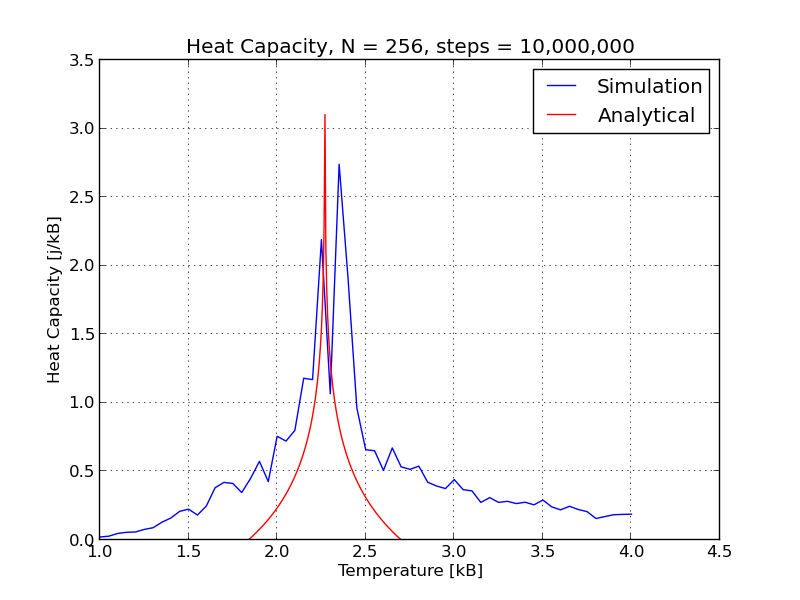
\includegraphics[width=0.5\textwidth]{cv_anal.png}
  \caption{The heat capacity derived from a series of simulations using a
  system of 256x256 spins and 10,000,000 steps,
  compared to an analytical approximation around the critical temperature.}
  \label{fig:heat}
\end{figure}


\begin{figure}[p]
  \centering
  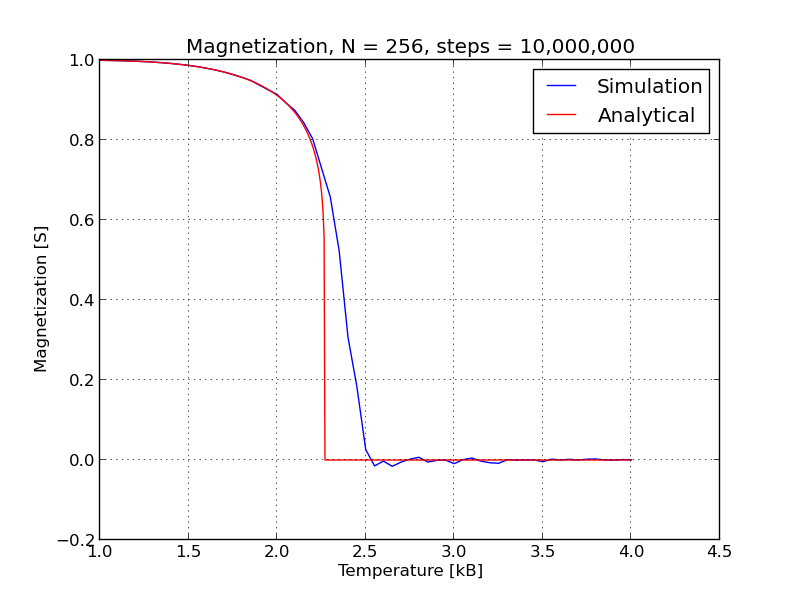
\includegraphics[width=0.5\textwidth]{mag_anal.png}
  \caption{The magnetization derived from a series of simulations using a system of
  256x256 spins and 10,000,000 steps, compared to the analytical solution.}
  \label{fig:magnetization}
\end{figure}


\subsection{Calculate the magnetic susceptibility}

After each iteration, save the magnetization and squared magnetization.
When your simulation is over, calculate the mean values and use these to calculate the magnetic susceptibility.
If you run a 20x20 lattice for 100,000 steps at $T = 1.5$ you should get $\chi$ values between $5 \cdot 10^{-5}$ and $8 \cdot 10^{-5}$.
There will be some variation in the numbers you get, so run the simulation a few times and record the average.
Again, remember that a proper burn-in period is required.\\

The magnetic susceptibility has a divergence around $T_c = 2.269$ - see Figure \ref{fig:susceptibility}.
If you run your simulation around this value, the results will vary quite a bit.

\begin{figure}[p]
  \centering
  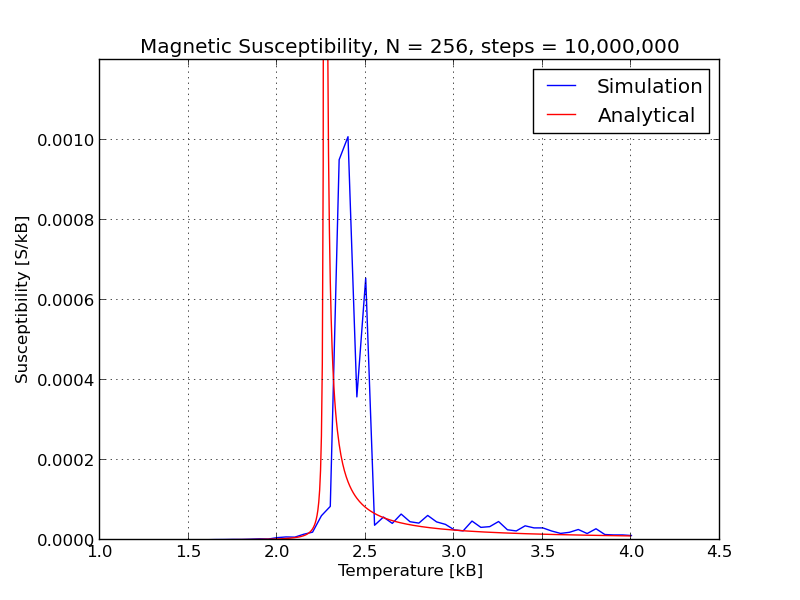
\includegraphics[width=0.5\textwidth]{xi_anal.png}
  \caption{The magnetic susceptibility derived from a series of simulations using a
  system of 256x256 spins and 10,000,000 steps, compared to an analytical approximation.}
  \label{fig:susceptibility}
\end{figure}

%\clearpage
\section{Data}

In addition to a brief presentation of the theory and your implementation of the 2D Ising mode,
you have to discuss the following results:

\begin{enumerate}
    \item Investigate how the size of your lattice, the burn-in period before you record $E$ and $M$ values, and the simulation lengths affect the calculated values.

    \item Run a long simulation at the critical temperature $T_c = 2.269$ and make a plot of the magnetization and energy for each iteration step.
      You should be able to observe that the total magnetizations can change back and forth from 1 to -1. Run the same simulation, but at $T= 1.0$ and $T = 3.5$ and compare.

    \item Run your simulation at different temperatures and make a plot of the heat capacity, magnetization and magnetic susceptibility versus the temperature.
    Do you observe a divergences around $T = 2.269$? You might have to run the same simulations more than once since there can be a substantial statistical variation in the values you obtain for $C_v$, $M$ and $\chi$.
\end{enumerate}


% ***************************************************
% END DOCUMENT
% ***************************************************

\end{document}
